\chapter{About the author}
\phantom{me}\hfill 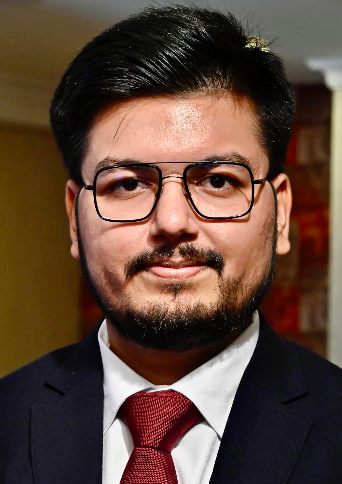
\includegraphics[height=25mm]{FiguresMisc/Vatsal.pdf}\\ %latex does not supprot jpg, insert a pdf version of your profile photo if you like...
\vspace{5mm}

These are the last two pages of my Ph.D. thesis where I am supposed to write about myself. Before doing so, I must admit that it is a herculean task, but I will try my best to share my story with you.

I was born on February 5th, 1996, in Laheriasarai, a small town in Bihar, India. As a kid, my first love was reading stories, which soon became a love for history. If I were not a fluid dynamicist today, I would probably have been a historian. The only problem was that I could only read stories about others and not write one of my own, which is another of my passions. Apart from reading, I also love collecting books. Ever since childhood, I have maintained a healthy collection of books, both antique and modern. 

Thanks to one of these books, I stumbled into the fascinating world of Physics. I remember getting puzzled by a question that seemed like a paradox at the time. I still remember the question. {\it To pull a cart, a horse applies a force on it. However, Newton's third law dictates that the cart applies an equal and opposite force on the horse. If we take the horse and the cart as a system, the net force on this system is zero. Then, how does a horse pull a cart?} It took me an entire sleepless night to come up with an answer, ending in a midnight call to my secondary school Physics teacher. 

The satisfaction of coming up with the correct answer set me up on this journey which led me to do a bachelors in Mechanical Engineering from the Indian Institute of Technology Roorkee, during which I worked as an undergraduate researcher with Prof. A. K. Das in the two-phase flow lab. I also did an internship with Prof. M. Bourgoin, Prof. J-P. Matas, and Prof. J. J. Jerome. This internship introduced me to the rich European research culture and the fluid dynamics community. The style of asking questions and exploring the fundamental fluid dynamics of everyday flows appealed to me. Subsequently, I decided to switch my bachelor's program to an integrated dual degree. I finished my master's thesis with Prof. Das. These works led me to pursue a doctoral work with Prof. D. Lohse in the Physics of Fluids group, where I have spent the last four years working on this Ph.D. thesis. 

But the story is not over yet. In the future, I want to continue this quest in the world of fluid dynamics by asking relevant questions and answering them to the best of my abilities. I also want to read more books and contribute to spreading the beautiful world of fluid dynamics to everyone. One day, I would also like to run a marathon, thanks to my recently acquired love for running. 



